\documentclass[10pt,a4paper]{article}
\usepackage[margin=21mm,headheight=14pt]{geometry}
\usepackage[T1]{fontenc}
\usepackage{lmodern,microtype,amsmath,booktabs,tabularx,array}
\usepackage[dvipsnames]{xcolor}
\usepackage{graphicx,pgfplots}
\pgfplotsset{compat=1.18}
\usepackage{fancyhdr}
\usepackage[colorlinks=true,linkcolor=MidnightBlue,urlcolor=MidnightBlue]{hyperref}
\pagestyle{fancy}\fancyhf{}
\fancyhead[L]{\small Mihal Dimo / Qwen3.8-27B on H100}
\fancyhead[R]{\small 1 October 2026}
\fancyfoot[C]{\small\thepage}
\setlength{\parindent}{0pt}\setlength{\parskip}{5pt}
\renewcommand{\arraystretch}{1.15}
\newcommand{\MicroBase}{1581.29}
\newcommand{\MicroCustom}{698.91}
\newcommand{\MicroSpeedup}{2.26}
\newcommand{\PrefillKernelGain}{+5.90}
\newcommand{\DecodeKernelGain}{+0.93}
\newcommand{\NumericalCases}{216}
\newcommand{\CustomProfileCalls}{1408}
\newcommand{\MicroRows}{1 & 2.00 & 2.09 & 0.96$\times$ \\
32 & 4.85 & 3.17 & 1.53$\times$ \\
64 & 7.57 & 4.60 & 1.65$\times$ \\
256 & 27.07 & 13.70 & 1.98$\times$ \\
1,024 & 100.61 & 46.25 & 2.18$\times$ \\
4,096 & 394.71 & 175.77 & 2.25$\times$ \\
8,192 & 791.88 & 350.89 & 2.26$\times$ \\
16,384 & 1581.29 & 698.91 & 2.26$\times$ \\}
\newcommand{\EngineRows}{Single / output tok/s & 72.56 & 72.45 & -0.15\% \\
Prefill / input tok/s & 18127.41 & 19196.34 & +5.90\% \\
Decode / output tok/s & 1645.49 & 1660.77 & +0.93\% \\
Mixed / output tok/s & 992.28 & 1028.54 & +3.65\% \\}
\newcommand{\LatencyRows}{Single & 96.99 & 101.12 & 13.14 & 13.14 \\
Prefill & 8165.14 & 7513.16 & --- & --- \\
Decode & 334.95 & 327.06 & 17.00 & 16.89 \\
Mixed & 1899.64 & 1786.43 & 18.26 & 18.18 \\}
\newcommand{\TokenComparison}{259 of 400 matched measured requests have identical generated-token hashes. Two unchanged reference runs agree on 264/400 requests. Thus the full engine is not bitwise deterministic in these runs. This control does not prove all differences are harmless or caused by scheduling; representative quality evaluation remains necessary. Both configurations pass the same three text smoke checks with identical answers.}

\title{\vspace{-10mm}\textbf{A Warp-Level SiLU--FP8 Kernel for Qwen3.8-27B}\\[3pt]
\large Profiling, numerical validation, and serving tradeoffs on an H100}
\author{Mihal Dimo\\\small\href{https://github.com/mhdimo/qwen38-h100-lab}{github.com/mhdimo/qwen38-h100-lab}}
\date{1 October 2026}
\begin{document}
\maketitle\thispagestyle{fancy}\vspace{-6mm}
\begin{abstract}
Following the serving-configuration study, we implement and test a custom CUDA
kernel for fused SiLU activation, multiplication and per-group FP8 quantization.
The target is selected from actual GPU profiles of Qwen3.8-27B-FP8 on an H100.
The candidate preserves the installed vLLM operator's numerical format and
matches its FP8 output bytes and FP32 scales over the tested numerical matrix.
At the largest tested prefill shape, average per-operation CUDA-graph replay time
falls from \MicroBase{} to \MicroCustom{} microseconds (\MicroSpeedup{}$\times$).
The full-model prefill-heavy throughput change is \PrefillKernelGain{}\%, while
decode-heavy throughput changes by \DecodeKernelGain{}\%.
These incremental gains compare two otherwise matched, already-tuned engines;
they are separate from the earlier large gain due to enabling concurrency.
\end{abstract}

\section{Measurement-driven target selection}
This is the third pass of a single-H100 study of a Qwen3.8-27B-FP8 vLLM
deployment; the earlier serving-configuration report (\texttt{paper.pdf}) and
the Gated DeltaNet ablation (\texttt{gdn.pdf}) accompany it in this repository.
The hardware is an isolated NVIDIA H100 80GB HBM3, with driver 610.57.04 and a
700 W power limit. The pinned stack is vLLM 0.26.0, PyTorch 2.11.0 and Triton 3.6.0.
CUDA 13.2 compiles the new source for SM90. Model revision is
\texttt{017b9c7af6b5689d5dd426a76e0bc077eb5ca20a}; native FP8 weights and BF16
cache formats are unchanged. All experiments run in a separate lab worker.

We capture warmed prefill and decode workloads with the PyTorch GPU profiler.
For steady decode, we select GPU events sharing CUDA-graph launch correlation IDs
with the packed recurrent Gated DeltaNet kernel, excluding prompt processing.
The initial capture contains ten such decode graph launches. Kernel durations
are summed; their percentages are not exclusive fractions of wall-clock time.

\begin{center}\small
\begin{tabular}{@{}lrr@{}}\toprule
Selected operation & Prefill capture & Steady decode graphs \\\midrule
SiLU/multiply/FP8 quantization & 14.54\% & 2.10\% \\
Gated DeltaNet packed recurrence & --- & 20.45\% \\
\bottomrule\end{tabular}
\end{center}

This evidence makes activation quantization a useful first prefill target, while
identifying Gated DeltaNet recurrence as a larger remaining decode opportunity.
The custom-engine traces contain \CustomProfileCalls{} launches of the new kernel,
confirming actual dispatch inside vLLM. Merely registering a replacement is not
treated as evidence that the engine executed it. Profiled runs are excluded from
all serving-throughput comparisons.

\section{Kernel design and integration}
For each 128-element group of BF16 gate and up-projection values, compute
\[
 z_i=\operatorname{SiLU}(g_i)u_i,\qquad
 s=\max\left(\frac{\max_i|z_i|}{448},\frac{1}{448\cdot512}\right),\qquad
 q_i=\operatorname{E4M3}\!\left(\operatorname{clip}(z_i/s,-448,448)\right).
\]
An optional upper bound clamps the scale before its lower floor, matching the
installed operator. Arithmetic before the final cast is FP32.

In \texttt{custom\_kernels/silu\_mul\_fp8.cu}, one warp owns one quantization group
and each lane processes four adjacent values. Four warps process adjacent groups
per block. Warp shuffles reduce the maximum; packed stores write four FP8 bytes.
This removes the reference kernel's block-wide reduction barriers and shared
memory. The compiler reports 29 registers per thread, no spills and no barriers
for the custom kernel. These are compiler reports, not Nsight Compute counters.

The extension compiles before warmup and graph capture. An explicit lab worker
substitutes a separately registered operator in vLLM's activation-fusion mapping.
The installed packages are unchanged. Unsupported formats or pointer alignment
use the original operator; the native entry point checks its alignment contract.
Compact row-major and transposed scale layouts are supported. The measured
batch-one regression is avoided by retaining the original kernel for that case.

\section{Numerical validation}
The final suite covers \NumericalCases{} cases (168 nonempty and 48 empty-input
checks) across three seeds, empty inputs,
partial blocks, batch sizes through 1,024, Qwen's 17,408-wide intermediate, both
scale layouts, zeros, tiny/extreme finite values and scale saturation. The suite
requires identical FP8 bytes for nonempty inputs against the installed CUDA operator and scale
agreement at rtol $2\times10^{-6}$, atol $10^{-8}$; observed scale differences
were zero. An independent PyTorch formula checks the mathematical result.
Four CUDA-graph replays use changing inputs. Additional tests cover unaligned
storage-offset views and FP16 fallback. An initial fast-math build failed exact
FP8 comparison; removing that flag resolved the failure. Failed logs are retained.

\section{Microbenchmark and operation speedup}
Each measurement uses a warmed graph containing four operations on distinct
input buffers. CUDA events time 30 graph replays; execution order alternates
between implementations across ten trials. The table reports the median average
time per operation. Small shapes remain cache-resident; the input pool at the
largest shape is 4.56 GB. Timings include graph scheduling and any submission
gaps, and are not advertised as isolated instruction-level kernel latency.

\begin{center}\small
\begin{tabular}{@{}rrrr@{}}\toprule
Token rows & vLLM ($\mu$s) & Custom ($\mu$s) & Speedup \\\midrule
\MicroRows
\bottomrule\end{tabular}
\end{center}

\begin{figure}[h]
\centering
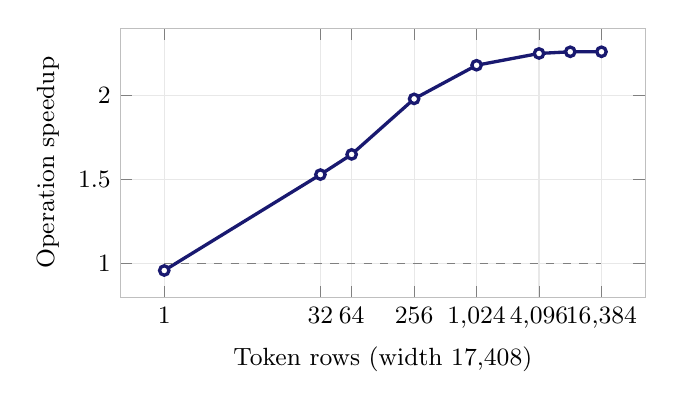
\begin{tikzpicture}
\begin{axis}[width=.68\linewidth,height=50mm,
  xlabel={Token rows (width 17,408)}, ylabel={Operation speedup},
  xmode=log, log basis x=2, xtick={1,32,64,256,1024,4096,16384},
  xticklabels={1,32,64,256,1{,}024,4{,}096,16{,}384},
  ymin=0.8, ymax=2.4, ytick={1.0,1.5,2.0},
  grid=major, grid style={gray!18}, axis line style={gray!50},
  tick label style={font=\small}, label style={font=\small},
  mark size=1.7pt]
\addplot[very thick,color=MidnightBlue,mark=*,mark options={fill=white}]
  coordinates {(1,0.96)(32,1.53)(64,1.65)(256,1.98)(1024,2.18)(4096,2.25)(8192,2.26)(16384,2.26)};
\addplot[dashed,gray] coordinates {(1,1)(16384,1)};
\end{axis}
\end{tikzpicture}
\caption{Warmed CUDA-graph operation speedup (custom vs.\ installed kernel).
At the smallest shape the candidate is slightly slower, so the serving adapter
selects the original kernel there.}
\end{figure}

All rows use width 17,408 and transposed FP32 scales. Batch one regresses slightly
in the standalone candidate; the serving adapter selects the original kernel
there. No weight compression or reduced numerical tolerance is used for speed.

\newpage
\section{Matched end-to-end comparison}
The reference is the previously tuned engine: 64 sequence capacity, 16 GiB cache,
16,384 scheduled tokens, chunked prefill, asynchronous scheduling and
\texttt{FULL\_AND\_PIECEWISE} CUDA graphs. The candidate changes the activation
kernel through the lab worker and uses a separate compilation cache. Compilation,
model loading and shape warmup are excluded from timing.

Both configurations complete 400 requests: two repetitions each of 128/128
tokens at concurrency one, 4096/1 at concurrency 32, 128/128 at concurrency 32,
and 1024/128 at concurrency 32. Prompt token IDs and output lengths are fixed and
matched. The harness enforces completed outputs and no prefix-cache hits.

\begin{center}\small
\begin{tabular}{@{}lrrr@{}}\toprule
Workload / throughput metric & Tuned vLLM & Custom kernel & Change \\\midrule
\EngineRows
\bottomrule\end{tabular}
\end{center}

\begin{center}\small
\begin{tabular}{@{}lrrrr@{}}\toprule
& \multicolumn{2}{c}{TTFT p95 (ms)} & \multicolumn{2}{c}{TPOT p95 (ms)}\\
Workload & vLLM & Custom & vLLM & Custom\\\midrule
\LatencyRows
\bottomrule\end{tabular}
\end{center}
TTFT includes queueing. TPOT is each request's mean interval after the first
output, not an individual-token tail metric. Single-output requests have no TPOT.
\TokenComparison

\section{Limits and reproducibility}
This is a measured first kernel experiment, not an exhaustive optimization of
the H100 or a production deployment. Two sequential repetitions, synthetic
lengths and unconstrained GPU clocks limit generalization and confidence in small
differences. The three text smoke checks do not establish multimodal or
structured-output quality. The application still has its original admission
policy; direct AsyncLLM throughput does not measure production HTTP capacity.

The accompanying \texttt{kernel\_data.json} records source paths, hashes,
per-repetition rates and numerical results. \texttt{kernel\_build\_data.py}
regenerates every tabulated number. Raw traces, failed attempts, final CUDA source
and build products are preserved in the local archive. The temporary lab
workspace on the H100 host was removed after hash-verified transfer; no
production files were modified.

\small
\textbf{Commands (on the H100 host):}
\begin{verbatim}
python run_suite.py --kernel-action validate
python run_suite.py --kernel-action bench
python run_suite.py --configs batch64_t16384 \
  batch64_t16384_custom_silu --repetitions 2
\end{verbatim}
\textbf{Reference implementation:}
\href{https://github.com/vllm-project/vllm/blob/main/csrc/libtorch_stable/quantization/fused_kernels/fused_silu_mul_block_quant.cu}{vLLM CUDA activation/quantization source}.
Upstream source explains the operation; the installed v0.26.0 binary is the
numerical and performance oracle. The earlier serving study remains in
\texttt{paper.pdf} and the GDN ablation in \texttt{gdn.pdf}; their gains must
not be attributed to this kernel.
\end{document}
